% Options for packages loaded elsewhere
% Options for packages loaded elsewhere
\PassOptionsToPackage{unicode}{hyperref}
\PassOptionsToPackage{hyphens}{url}
\PassOptionsToPackage{dvipsnames,svgnames,x11names}{xcolor}
%
\documentclass[
  11pt,
  letterpaper,
  DIV=11,
  numbers=noendperiod]{scrartcl}
\usepackage{xcolor}
\usepackage[margin=1.1in,footskip=0.35in]{geometry}
\usepackage{amsmath,amssymb}
\setcounter{secnumdepth}{-\maxdimen} % remove section numbering
\usepackage{iftex}
\ifPDFTeX
  \usepackage[T1]{fontenc}
  \usepackage[utf8]{inputenc}
  \usepackage{textcomp} % provide euro and other symbols
\else % if luatex or xetex
  \usepackage{unicode-math} % this also loads fontspec
  \defaultfontfeatures{Scale=MatchLowercase}
  \defaultfontfeatures[\rmfamily]{Ligatures=TeX,Scale=1}
\fi
\usepackage{lmodern}
\ifPDFTeX\else
  % xetex/luatex font selection
\fi
% Use upquote if available, for straight quotes in verbatim environments
\IfFileExists{upquote.sty}{\usepackage{upquote}}{}
\IfFileExists{microtype.sty}{% use microtype if available
  \usepackage[]{microtype}
  \UseMicrotypeSet[protrusion]{basicmath} % disable protrusion for tt fonts
}{}
\makeatletter
\@ifundefined{KOMAClassName}{% if non-KOMA class
  \IfFileExists{parskip.sty}{%
    \usepackage{parskip}
  }{% else
    \setlength{\parindent}{0pt}
    \setlength{\parskip}{6pt plus 2pt minus 1pt}}
}{% if KOMA class
  \KOMAoptions{parskip=half}}
\makeatother
% Make \paragraph and \subparagraph free-standing
\makeatletter
\ifx\paragraph\undefined\else
  \let\oldparagraph\paragraph
  \renewcommand{\paragraph}{
    \@ifstar
      \xxxParagraphStar
      \xxxParagraphNoStar
  }
  \newcommand{\xxxParagraphStar}[1]{\oldparagraph*{#1}\mbox{}}
  \newcommand{\xxxParagraphNoStar}[1]{\oldparagraph{#1}\mbox{}}
\fi
\ifx\subparagraph\undefined\else
  \let\oldsubparagraph\subparagraph
  \renewcommand{\subparagraph}{
    \@ifstar
      \xxxSubParagraphStar
      \xxxSubParagraphNoStar
  }
  \newcommand{\xxxSubParagraphStar}[1]{\oldsubparagraph*{#1}\mbox{}}
  \newcommand{\xxxSubParagraphNoStar}[1]{\oldsubparagraph{#1}\mbox{}}
\fi
\makeatother


\usepackage{longtable,booktabs,array}
\usepackage{calc} % for calculating minipage widths
% Correct order of tables after \paragraph or \subparagraph
\usepackage{etoolbox}
\makeatletter
\patchcmd\longtable{\par}{\if@noskipsec\mbox{}\fi\par}{}{}
\makeatother
% Allow footnotes in longtable head/foot
\IfFileExists{footnotehyper.sty}{\usepackage{footnotehyper}}{\usepackage{footnote}}
\makesavenoteenv{longtable}
\usepackage{graphicx}
\makeatletter
\newsavebox\pandoc@box
\newcommand*\pandocbounded[1]{% scales image to fit in text height/width
  \sbox\pandoc@box{#1}%
  \Gscale@div\@tempa{\textheight}{\dimexpr\ht\pandoc@box+\dp\pandoc@box\relax}%
  \Gscale@div\@tempb{\linewidth}{\wd\pandoc@box}%
  \ifdim\@tempb\p@<\@tempa\p@\let\@tempa\@tempb\fi% select the smaller of both
  \ifdim\@tempa\p@<\p@\scalebox{\@tempa}{\usebox\pandoc@box}%
  \else\usebox{\pandoc@box}%
  \fi%
}
% Set default figure placement to htbp
\def\fps@figure{htbp}
\makeatother


% definitions for citeproc citations
\NewDocumentCommand\citeproctext{}{}
\NewDocumentCommand\citeproc{mm}{%
  \begingroup\def\citeproctext{#2}\cite{#1}\endgroup}
\makeatletter
 % allow citations to break across lines
 \let\@cite@ofmt\@firstofone
 % avoid brackets around text for \cite:
 \def\@biblabel#1{}
 \def\@cite#1#2{{#1\if@tempswa , #2\fi}}
\makeatother
\newlength{\cslhangindent}
\setlength{\cslhangindent}{1.5em}
\newlength{\csllabelwidth}
\setlength{\csllabelwidth}{3em}
\newenvironment{CSLReferences}[2] % #1 hanging-indent, #2 entry-spacing
 {\begin{list}{}{%
  \setlength{\itemindent}{0pt}
  \setlength{\leftmargin}{0pt}
  \setlength{\parsep}{0pt}
  % turn on hanging indent if param 1 is 1
  \ifodd #1
   \setlength{\leftmargin}{\cslhangindent}
   \setlength{\itemindent}{-1\cslhangindent}
  \fi
  % set entry spacing
  \setlength{\itemsep}{#2\baselineskip}}}
 {\end{list}}
\usepackage{calc}
\newcommand{\CSLBlock}[1]{\hfill\break\parbox[t]{\linewidth}{\strut\ignorespaces#1\strut}}
\newcommand{\CSLLeftMargin}[1]{\parbox[t]{\csllabelwidth}{\strut#1\strut}}
\newcommand{\CSLRightInline}[1]{\parbox[t]{\linewidth - \csllabelwidth}{\strut#1\strut}}
\newcommand{\CSLIndent}[1]{\hspace{\cslhangindent}#1}



\setlength{\emergencystretch}{3em} % prevent overfull lines

\providecommand{\tightlist}{%
  \setlength{\itemsep}{0pt}\setlength{\parskip}{0pt}}



 


\KOMAoption{captions}{tableheading,figureheading}
\allowdisplaybreaks
\usepackage{setspace}\setstretch{1.1}
\usepackage{etoolbox} \newcommand{\zerodisplayskips}{ \setlength{\abovedisplayskip}{2pt} \setlength{\belowdisplayskip}{2pt} \setlength{\abovedisplayshortskip}{1pt} \setlength{\belowdisplayshortskip}{1pt}} \appto{\normalsize}{\zerodisplayskips} \appto{\small}{\zerodisplayskips} \appto{\footnotesize}{\zerodisplayskips}
\usepackage{pgf}\usepackage{pgfplots}\usepackage{tikz}
\usetikzlibrary{graphs, arrows, automata, shadings}
\setlength{\floatsep}{0pt}
\usepackage{enumitem}\setlist[enumerate]{leftmargin=*}
\usepackage{verbatim}
\makeatletter \patchcmd{\@verbatim}{\verbatim@font}{\singlespacing\small\verbatim@font}{}{}
\RedeclareSectionCommand[runin=false, beforeskip=-1sp, afterskip=-0.1\baselineskip]{section}
\RedeclareSectionCommand[runin=false, beforeskip=-1sp, afterskip=-0.1\baselineskip]{subsection}
\newcommand\blfootnote[1]{ \begingroup \renewcommand\thefootnote{}\footnote{#1} \addtocounter{footnote}{-1} \endgroup}
\setlength{\columnsep}{2em}
\setlength{\tabcolsep}{2pt}
\usepackage{dsfont}
\usepackage[section]{placeins}
\makeatletter
\@ifpackageloaded{float}{}{\usepackage{float}}
\floatstyle{plain}
\@ifundefined{c@chapter}{\newfloat{suppfig}{h}{losuppfig}}{\newfloat{suppfig}{h}{losuppfig}[chapter]}
\floatname{suppfig}{Figure S}
\floatstyle{plaintop}
\restylefloat{suppfig}
\newcommand*\quartosuppfigref[1]{Figure \hyperref[#1]{S\ref{#1}}}
\@ifpackageloaded{caption}{}{\usepackage{caption}}
\DeclareCaptionLabelFormat{quartosuppfigreflabelformat}{#1#2}
\captionsetup[suppfig]{labelformat=quartosuppfigreflabelformat}
\newcommand*\listofsuppfigs{\listof{suppfig}{List of Supplemental Figures}}
\makeatother
\makeatletter
\@ifpackageloaded{float}{}{\usepackage{float}}
\floatstyle{plain}
\@ifundefined{c@chapter}{\newfloat{supptbl}{h}{losupptbl}}{\newfloat{supptbl}{h}{losupptbl}[chapter]}
\floatname{supptbl}{Table S}
\floatstyle{plaintop}
\restylefloat{supptbl}
\newcommand*\quartosupptblref[1]{Table \hyperref[#1]{S\ref{#1}}}
\@ifpackageloaded{caption}{}{\usepackage{caption}}
\DeclareCaptionLabelFormat{quartosupptblreflabelformat}{#1#2}
\captionsetup[supptbl]{labelformat=quartosupptblreflabelformat}
\newcommand*\listofsupptbls{\listof{supptbl}{List of Supplemental Tables}}
\makeatother
\makeatletter
\@ifpackageloaded{caption}{}{\usepackage{caption}}
\AtBeginDocument{%
\ifdefined\contentsname
  \renewcommand*\contentsname{Table of contents}
\else
  \newcommand\contentsname{Table of contents}
\fi
\ifdefined\listfigurename
  \renewcommand*\listfigurename{List of figures}
\else
  \newcommand\listfigurename{List of figures}
\fi
\ifdefined\listtablename
  \renewcommand*\listtablename{List of tables}
\else
  \newcommand\listtablename{List of tables}
\fi
\ifdefined\figurename
  \renewcommand*\figurename{Figure}
\else
  \newcommand\figurename{Figure}
\fi
\ifdefined\tablename
  \renewcommand*\tablename{Table}
\else
  \newcommand\tablename{Table}
\fi
}
\@ifpackageloaded{float}{}{\usepackage{float}}
\floatstyle{ruled}
\@ifundefined{c@chapter}{\newfloat{codelisting}{h}{lop}}{\newfloat{codelisting}{h}{lop}[chapter]}
\floatname{codelisting}{Listing}
\newcommand*\listoflistings{\listof{codelisting}{List of Listings}}
\makeatother
\makeatletter
\makeatother
\makeatletter
\@ifpackageloaded{caption}{}{\usepackage{caption}}
\@ifpackageloaded{subcaption}{}{\usepackage{subcaption}}
\makeatother
\usepackage{bookmark}
\IfFileExists{xurl.sty}{\usepackage{xurl}}{} % add URL line breaks if available
\urlstyle{same}
\hypersetup{
  colorlinks=true,
  linkcolor={blue},
  filecolor={Maroon},
  citecolor={Blue},
  urlcolor={Blue},
  pdfcreator={LaTeX via pandoc}}


\author{}
\date{}
\begin{document}


\section{Hypothetical interventions on workplace exposure with
guaranteed
positivity}\label{hypothetical-interventions-on-workplace-exposure-with-guaranteed-positivity}

\subsection{Abstract}\label{abstract}

Non-Hodgkin lymphoma (NHL) incidence was recently linked to exposure to
metalworking fluid (MWF) in a standard survival analysis of the United
Auto Workers-General Motors cohort. To provide results more directly
relevant to guiding exposure limits, we estimated the counterfactual
risks of NHL under hypothetical supportable interventions on exposure to
MWF in the same cohort (n = 33,134) for 1985-2015 using the
hazard-extended iterative conditional expectation g-formula. We
addressed potential bias due to the healthy worker survivor effect while
investigating stochastic dynamic interventions that avoid extrapolation
beyond observed conditional exposure distributions, thus guaranteeing
positivity by design. These interventions reduced exposures above
specified target limits to the nearest supported level of exposure but
allowed exposures below the limit to vary naturally. 339 NHL cases
occurred over the 30-year follow-up period. Stronger target limits on
MWF exposure resulted in monotonic reductions in NHL risk. Setting the
target exposure limit at 0.5 mg/m\textsuperscript{3}, the NIOSH
recommended exposure limit, would have prevented 124 (95\% CI: 66, 202)
cases. We expect that uniformly enforcing the target exposure limits,
regardless of data support, would have yielded even stronger protective
effects. Strengthening protections against exposure to MWF may protect
workers from NHL during the anticipated boom in domestic manufacturing.

\newpage{}

\subsection{Introduction}\label{introduction}

Non-Hodgkin Lymphoma (NHL) incidence in the United States doubled
between 1973 and 1994 before plateauing at around 19 per 100,000 persons
per year, making it the seventh most common cancer in the country
{[}1,2{]}. The strongest known risk factors of NHL are autoimmune
disease and immunosuppression {[}3,4{]}. The relationship between
autoimmune diseases NHL is specific in that each disease is associated
with a particular subtype of NHL {[}5{]}. Immunosuppression and
infection with HIV are strongly associated with Burkitt lymphoma
{[}5{]}. These risk factors cannot fully explain the historic rise or
present burden of NHL, however {[}6{]}. Since the rise in NHL incidence
coincided with a period of rapid and extensive chemicalization in
industry, agriculture and warfare; environmental and occupational
exposures may play an important explanatory role in the epidemiology of
NHL {[}7,8{]}. Existing epidemiologic studies suggest that occupational
exposures may increase the risk of NHL without subtype specificity
{[}5{]}.

Pesticide exposure among workers in agricultural settings was a common
target of NHL research in recent decades. A meta-analysis of 44 articles
published between 1980 and 2014 found statistically significant
associations between NHL and exposure to several classes of pesticides
including carbamate, organophosporus, triazine, and organochlorine
{[}9{]}. Occupational exposures associated with NHL are not limited to
the agricultural sector, however. Occupational groups associated with
NHL risk also include metal processors, health workers, salespeople,
machinists, and electricians {[}2,10,11{]}. Workers in these
occupational groups often come into contact with industrial chemicals
such as gasoline, solvents, coolants, and lubricants such as
metalworking fluids (MWF).

Metalworking fluids are complex mixtures of oil, water, and chemical
additives that cool and lubricate metal machining operations. There are
three general types of MWF: straight, soluble, and synthetic. During
shaping, grinding, and cutting operations, MWFs are misted, poured, or
blasted at high pressure onto work surfaces to remove debris, cool
metal, improve efficiency, and prevent deterioration of tools. Although
MWFs are essential to manufacturing processes, they also present a
potential health hazard to exposed workers through inhalation or
ingestion of MWF particulate mass. In response to health concerns
related to the carcinogenicity of polycyclic aromatic hydrocarbons
(PAHs) in mineral oil as well as the rising global cost of oil products,
water-based soluble MWF, which usually contain about 40-70\% oil by
weight, were developed to replace oil-based straight MWF {[}12--14{]}.
Today, soluble MWF is the most common type of MWF in metal machining
operations {[}15{]}.

One challenge in estimating the causal effects of occupational exposures
on worker health is the Healthy Worker Survivor Effect (HWSE), the
process by which healthier individuals remain at work where they
accumulate more exposure while those more susceptible to the deleterious
health effects of exposure leave work {[}16{]}. The parametric g-formula
is an early causal inference method in statistics developed to estimate
causal effects in longitudinal observational studies where the HWSE or
other forms of time-varying confounding/selection bias affected by past
exposure may be operating {[}17--19{]}. A central requirement necessary
for causal inference from observational data is positivity (overlap),
\emph{i.e.,} adequate variation in the exposure of interest within
strata formed by confounder and exposure histories {[}20{]}.

When positivity is not satisfied, causal inference methods that rely
only on models for the counterfactual outcome, and not the treatment
mechanism, may still yield valid causal estimates, if the models are
correctly specified. We evaluated how hypothetical interventions on
exposure to soluble MWF would affect the incidence of NHL between 1985
and 2015 in the United Auto Workers-General Motors (UAW-GM) occupational
cohort using the iterative conditional expectation (ICE) parametric
g-formula, which relies on models for the outcome only. To further
address potential violations in positivity, we defined and evaluated
hypothetical interventions resulting in post-intervention exposure
histories whose propensity score is strictly greater than zero
\emph{i.e.}, exposure histories that can be found in the observed data.
We call these hypothetical interventions ``supportable''.

\subsection{Methods}\label{methods}

We estimated the cumulative incidence of NHL between 1985 and 2015 under
supportable interventions based on selected target exposure limits on
annual average daily exposure to soluble MWF by applying the
hazard-extended ICE parametric we estimated the expected number of NHL
cases that we would observe if there were no censoring and no limit on
exposure. Then, we contrasted this case count to that under supportable
interventions based on five hypothetical target exposure limits and no
censoring. The five target exposure limits were (1) 2.0, (2) 1.0, (3)
0.5, (4) 0.25, and (5) 0.05 mg/m\textsuperscript{3}. The National
Institute for Occupational Safety and Health (NIOSH) recommended
exposure limit (REL) for time-weighted average total particulate mass
(PM) composed of MWF is 0.5 mg/m\textsuperscript{3} {[}21{]}.

For each target exposure limit, period of follow-up, and stratum defined
by unique combinations of confounder and exposure histories, we found a
supportable exposure limit, which was the maximum observed value of
exposure at or below the target exposure limit, if such a value exists.
If all of the observed values were above the target limit, the
supportable limit was the minimum observed value. The supportable
intervention rule then reduces exposures above the supportable exposure
limit to that limit, but allows exposures at or below the limit to vary
according to their observed distribution. Applying the supportable
intervention rule to the observed distribution of exposure produces the
intervention distribution that defines the corresponding stochastic
dynamic intervention with guaranteed positivity. We estimated the effect
of supportable intervention rules based on the selected target exposure
limits, expressed as stochastic dynamic interventions, using the
hazard-extended ICE parametric g-formula {[}22{]}.

Figure 1 presents three example scenarios where the target exposure
limit is 0.25 mg/m\textsuperscript{3} in all cases, but the supportable
exposure limit differs depending on what the observed data supports. In
Figure 1a, the supportable exposure limit is equal to the target
exposure limit as some individuals with that particular set of potential
confounder and exposure histories were observed to have experienced
exposure at that level. In Figure 1b, the supportable exposure limit is
below the target exposure limit. In Figure 1c, the supportable exposure
limit, the minimum observed level of exposure in that stratum, is
greater than the target exposure limit.

\subsubsection{Study population}\label{study-population}

We used data from the UAW-GM cohort study, which included all hourly
workers at three automobile manufacturing plants in Michigan who had
worked at least three years by 1985. Past papers provide detailed
descriptions of the cohort {[}23,24{]}. The large size of the study
population and rich time-varying, quantitative MWF exposure data enable
the study of a relatively rare cancer and evaluation of realistic
interventions on MWF exposure in a longitudinal cohort setting. The
present study population (N = 33,134) was restricted to the autoworkers
who were at work in 1941 or not yet hired, missing no more than half of
their employment history, and still alive at the start of follow-up for
cancer incidence on January 1, 1985. Autoworkers in the study population
were followed until NHL diagnosis, death, December 31, 2014, or the
oldest observed age at death, whichever came earlier.

\subsubsection{Outcome and potential
confounders}\label{outcome-and-potential-confounders}

We identified incident cancers in the UAW-GM cohort between 1985 and
2014 by linkage to the Michigan Cancer Registry (MCR). Workers at Plants
1 and 2, located in the greater Detroit metropolitan area, were also
linked to the Detroit Regional Registry of the Surveillance,
Epidemiology, and End Results (SEER) Program. Cancer types were
distinguished using site and histology codes conforming to the
International classification of Diseases for Oncology,
3\textsuperscript{rd} edition (ICD-O-3). Non-Hodgkin lymphoma was
defined by cancers with any of the following ICD-O-3 histology codes:
9590-9597, 9670-9671, 9673, 9675, 9678-9680, 9684, 9687-9691, 9695,
9698-9702, 9705, 9708-9709, 9712, 9714-9719, 9724-9729, 9735, 9737-9738,
9811-9818, 9823, 9827, 9837. Details regarding cancer incidence
follow-up are described elsewhere {[}25{]}. Vital status was ascertained
from company records and by linkage to Social Security Administration,
National Death Index, and state mortality files.

Potential confounders including year of hire, sex, race, time off work,
employment status, and plant location were obtained from company
records. Race was missing for about 16\% of the cohort, most commonly
among workers hired before 1960 in Plant 2. In analyses, missing race
was considered a distinct category. All potential confounders were coded
as categorical variables. Cut-points for categorizing continuous
covariates were determined according to the quantiles among cases.

\subsubsection{Exposure}\label{exposure}

Quantitative measurement of time-varying MWF exposure is a
distinguishing strength of the UAW-GM cohort study relative to other
environmental or occupational health studies. Exposure assessment was
based on direct air sampling as well as company records. Company
industrial hygienists collected several hundred personal and area
samples for total particulate mass (mg/m\textsuperscript{3}) composed of
MWF over many decades. Research industrial hygienists collected
additional air sampling data when the cohort study was launched in the
mid 1980s {[}26,27{]}. These additional data combined with historical
data and company records were used to construct a job-exposure matrix of
quantitative 8-hour time-weighted average daily exposure estimates to
soluble, straight, and synthetic MWF for each combination of job,
department, and plant over time {[}28{]}. Workers' annual average daily
exposure to each MWF type was determined by combining this job-exposure
matrix with employment records, which recorded time-varying job type,
department, and plant for each employee from hire to termination or
1995, whichever came sooner. For employment records that were at least
half complete, gaps in the record were interpolated by carrying forward
the last known job type. The exposure assessment is described in detail
elsewhere {[}26,28,29{]}.

In previous analyses of NHL, exposure lags of 1 to 20 years were applied
to account for disease latency; we lagged cumulative MWF exposures by 20
years {[}30--32{]}. In analyses, MWF exposure history at start of
follow-up was summarized as the cumulative sum of average exposure
intensities. Exposure was coded as categorical variables with cut-points
at zero and the quintiles of nonzero exposure among cases. We estimated
the effects of hypothetical interventions on soluble MWF, the type of
MWF used most widely and in the greatest quantities while treating
co-exposure to straight and synthetic MWFs as potential confounders.

\subsubsection{Hazard-extended ICE parametric
g-formula}\label{hazard-extended-ice-parametric-g-formula}

We split the 30-year follow-up period into ten time periods based on the
deciles of the dates of diagnosis of NHL. The number of years per period
ranged from two to four. The hazard-extended ICE parametric g-formula
involves two stages. In the first, we estimate counterfactual discrete
hazards over the person-periods. In the second, we pool those estimates
to estimate the counterfactual risk over the entire follow-up period.
During pooling, we iteratively combine estimates of the counterfactual
hazard to obtain a pooled estimate over an increasing number of periods
starting from the last period. In each iteration, we perform model-based
standardization over exposure and covariate histories before combining
the counterfactual discrete hazard estimate with the estimated hazard
pooled over subsequent periods. This iterative process results in a
sequentially standardized estimate of the counterfactual cumulative
incidence of NHL when the intervention of interest is enforced over all
follow-up periods.

We investigated supportable interventions that guarantee positivity:
every value of exposure that could be assigned under our stochastic
dynamic intervention has propensity score strictly greater than zero. We
treated co-exposure to straight and synthetic MWF, employment status,
cumulative time off, age, duration of employment, sex (male/female),
race (Black/white/unknown), and plant (Plant 1/Plant 2/Plant 3) as
potential confounders. Exposure to MWF, employment status, time off, and
duration of employment were lagged 20 years. An overview of the general
steps of the estimation procedure are presented below. Note that we
refer to discrete hazards simply as hazards.

\begin{enumerate}
\def\labelenumi{\arabic{enumi}.}
\item
  Fit a pooled logistic regression model for NHL on potential
  confounders and exposure over all at-risk person-periods.
\item
  Predict the hazard for each person-period for each possible level of
  exposure using the model from step 1.
\item
  Within strata formed by unique combinations of potential confounders
  and exposure, obtain the intervention distribution of exposure by
  applying the supportable intervention rule to the observed exposure
  distribution.
\item
  Within strata, estimate the counterfactual hazard for each
  person-period by taking a weighted sum of the predicted hazards from
  step 2.
\item
  Starting at the penultimate period of follow-up, estimate the pooled
  counterfactual hazard:

  \begin{enumerate}
  \def\labelenumii{\alph{enumii})}
  \tightlist
  \item
    Regress the counterfactual hazard pooled over all subsequent periods
    on all past potential confounders and exposures.
  \item
    Predict the pooled hazard for each person at risk at the start of
    the period and each possible level of exposure using the model from
    (a). Retrieve the predicted hazards from step 2. For each person and
    level of exposure, multiply the predicted pooled hazard by one minus
    the corresponding predicted hazard. Then, add the predicted hazard
    to the product.
  \item
    Within strata formed by potential confounder and exposure histories,
    obtain the intervention distribution of exposure by applying the
    intervention rule to the observed exposure distribution.
  \item
    Within strata, estimate the counterfactual hazard pooled over the
    present and subsequent periods for each person by taking a weighted
    sum of the predicted pooled hazards from (b).
  \item
    If the present period is not first period, set the reference period
    to the preceding period and return to (a).
  \end{enumerate}
\item
  Compute the counterfactual risk by averaging the pooled counterfactual
  hazards across all persons.
\end{enumerate}

To account for censoring, fit the models in step 1 and step 5a among
those who were not censored and obtain predicted hazards for all at-risk
person-periods, including those that were censored.

We estimated cumulative incidence under no intervention on soluble MWF
and under the supportable interventions based on the five selected
target exposure limits. We contrasted the cumulative incidence under the
supportable interventions to that under no intervention on exposure by
computing the risk difference per 10,000 and the cumulative incidence
ratios. Confidence intervals were computed using the basic nonparametric
bootstrap with 1000 Monte Carlo samples from the population at the start
of follow-up. All the necessary scripts used to reproduce the analyses
are available on \href{https://github.com/kvntchn/gm-nhl-ice}{GitHub}.

\subsection{Results}\label{results}

Table 1 presents summary statistics for the full study population and
among those diagnosed with NHL between 1985 and 2015. The cohort is
predominantly white (64\%) and male (86\%). Year of hire and age at hire
were approximately the same among those with NHL and the full study
population. Median lagged cumulative exposure to all three types of MWF
was higher among NHL cases. Soluble MWF were the most widely used type,
with approximately 88\% of workers ever exposed. Median cumulative
exposure among the exposed was approximately 6 times higher for soluble
than for straight MWF. Figure 2 shows median annual average daily
exposure to the three MWF types among exposed workers over calendar
time. Exposure to MWF generally followed a downward trend over time.

The observed number of NHL cases over the 30-year follow-up period was
339. Table 2 presents estimates of the counterfactual number of cases,
risk difference per 10,000, and cumulative incidence ratios contrasting
supportable interventions on exposure to soluble MWF based on different
target exposure limits and no censoring. Under an intervention
eliminating censoring, the estimated number of cases was 502 (95\% CI:
439, 555). Interventions based on stronger target exposure limits on
soluble MWF resulted in monotonically stronger reductions in the
estimated cumulative incidence of NHL. Setting the target exposure limit
at the NIOSH REL 0.5 mg/m\textsuperscript{3} would have averted 124
(95\% CI: 66, 202) NHL cases.

\subsection{Discussion}\label{discussion}

Although NIOSH concluded that there exists substantial evidence linking
MWF exposure to several different cancers including larynx, rectum,
pancreas, skin, scrotum, and bladder cancer, their REL of 0.5
mg/m\textsuperscript{3} for total particulate mass derived from any type
of MWF was based on nonmalignant respiratory health effects {[}21,33{]}.
Exposure limits stronger than the NIOSH REL may provide valuable health
protections not previously taken into account by policy makers. Using
the hazard-extended ICE parametric g-formula, we estimated the
counterfactual expected number of NHL cases from 1985 to 2015 in the
UAW-GM cohort if we enforced hypothetical supportable interventions on
soluble MWF based on five different target exposure limits and found a
monotonic exposure-dependent relationship where stronger target exposure
limits yielded lower NHL case count estimates.

The g-formula is a well-known approach in causal inference used for
estimating causal effects in the presence of time-varying confounding
affected by past exposure {[}17{]}. Standard representations of the
g-formula include (1) a non-iterated expectation over the joint density
of covariates, (2) the ICE over time, and (3) an inverse probability
weighted expectation. The classic parametric g-formula is a plug-in
estimator for the g-formula under its first, non-iterative,
representation. It involves the parametric modeling of the full joint
distribution of the confounders, exposure, and outcome for each time
point {[}18,34{]}. Counterfactual quantities under hypothetical
interventions of interest are computed from Monte Carlo samples from
distributions implied by the fitted parametric models. In longitudinal
settings, this approach often requires specifying and fitting large
number of models in order to satisfy the exchangeability assumptions
necessary for causal identification. Despite this limitation, analysts
often choose the parametric g-formula because of the intuitive way it
handles interventions on the natural value of exposure. However, these
causal estimands are not unique to the parametric g-formula. The
distribution of exposure produced by marginalizing intervention rules
over the observed distribution of exposure within strata formed by
potential confounder and exposure histories defines a corresponding
stochastic dynamic intervention, whose effects may be estimated using
various estimators {[}22,35--38{]}. Estimating causal effects of this
implied stochastic dynamic intervention is analogous to that of
interventions on the natural value of exposure {[}34{]}.

Estimators using the ICE representation of the g-formula are capable of
estimating effects of stochastic dynamic interventions. These ICE
g-formula estimators require modeling only the conditional distributions
of the outcome at each time. Hence, they require fewer parametric
assumptions than the classic parametric g-formula. Counterfactual
outcome estimates over the follow-up period are computed from
interval-specific conditional estimates by applying the tower rule of
expectation. Under the assumptions of conditional exchangeability at all
time points, positivity, counterfactual consistency, and correct model
specification, the hazard-extended parametric g-formula yields unbiased
estimates of counterfactual risk with greater statistical efficiency
than both propensity score-based estimators and the non-extended ICE
g-formula.

Correct model specification is a standard assumption in all parametric
and semi-parametric analyses. In causal analyses of longitudinal cohort
studies, ICE g-formula estimators are less common than the classic
parametric g-formula {[}39{]}. However, a major limitation of the
classic g-formula is the g-null paradox: the guaranteed misspecification
of parametric models resulting in the false rejection of the null
hypothesis when the null is true and when there is time-varying
confounding affected by past exposure {[}40,41{]}. As with all ICE
g-formula estimators, the estimator we applied is not subject to the
g-null paradox. Furthermore, since ICE g-formula estimators require
fewer parametric modeling requirements than the classic parametric
g-formula, correct model specification may be achieved (or approximated)
more readily.

The consistency assumption, also known as the
no-multiple-versions-of-treatment or stable unit treatment value
assumption, is that counterfactual outcomes under each possible exposure
value take on a unique value {[}42,43{]}. This assumption would be
violated if there were multiple versions of treatment causally
associated with different outcomes. This basic notion of consistency is
violated in our analysis because our exposure of interest is a complex
mixture of diverse components with substantial variation over time due
to changes in formulation as well as the natural physical, chemical, and
biological changes in the MWF over the course of its use and reuse
{[}44{]}. However, causal effect estimates under violations in the
consistency assumption are still valid and unbiased if there is adequate
adjustment for confounders of the exposure-version relationship
{[}43{]}. This may be thought of as conditional consistency within
strata, in which there is only one version of treatment. Our analysis
indexed time periods over calendar time and adjusted for age, year of
hire, and plant. In this way, we limited potential for bias due to
variation in MWF composition.

Positivity refers to the need for adequate variation in future exposure
among strata formed by observed covariate and intervention-compliant
exposure histories. Even under conditional exchangeability, where
exposures within these strata may be considered the result of
experimental assignment, expected counterfactual outcomes under
different exposures may not be estimable if there is excessive sparsity
in the observed distribution of exposures {[}45{]}. Rather than address
potential violations in positivity analytically, we investigated
stochastic dynamic interventions on soluble MWF exposure based on
intervention distributions which are nonzero only where the propensity
score is strictly positive. Hence, our supportable interventions
guarantee positivity. Interventions that guarantee positivity have been
suggested in the past and have also been called ``realistic''
interventions {[}20{]}.

Conditional exchangeability means that for all time points, there is no
confounding of the relationship between exposure/censoring and both
future exposure/censoring and NHL status given the observed past,
including past exposure and confounders {[}19,38{]}. A major threat to
conditional exchangeability in longitudinal occupational studies is the
HWSE. We limit potential bias due to the HWSE by conditioning on
cumulative exposure, employment status, and cumulative time off history
at each time point. Cumulative time off and employment status are
reasonable mediators of the causal paths linking past health to future
exposure and health, but adjustment for these variables may not be
sufficient for eliminating bias due to the HWSE. Declines in a worker's
health may lead to reductions in work-related exposure without affecting
employment status or time off work {[}46{]}. We expect the absence of
time-varying measures of worker health over the life course to result in
bias toward the null.

Much of the existing epidemiologic literature linking occupational and
environmental exposures to NHL report findings from case-control studies
where exposures are measured as binary indicators of exposure or as
membership in a particular occupational group {[}47--50{]}. Associations
between occupations and NHL risk vary considerably, but one study of
working men in Kansas and Nebraska found strong associations between NHL
risk and occupations involving metalworking and motor vehicles {[}51{]}.
Both of these occupations may entail exposure to soluble MWF, which
contain mineral oils and a number of chemical additives of concern for
human health and for NHL risk in particular. Organic compounds
containing phosphorous, chlorine, sulfur, nitrogen, and boron are
commonly added to soluble MWF to control microbial growth, improve
performance under high heat/pressure, and inhibit corrosion {[}52{]}.
Organophosphorus compounds include organophosphate pesticides, which
have been linked to cancer risk in epidemiologic and animal studies.
Some were classified as possibly carcinogenic by the IARC {[}53{]}.
Studies of occupational exposure to chlorinated solvents and pesticides
have also been linked to NHL risk {[}54--58{]}. In 2014, the IARC
classified trichloroethylene, tetrachloroethylene, and other chlorinated
agents as Group 1 carcinogens {[}59{]}. Chlorinated solvents are
commonly used as degreasers in industrial settings, but their use in the
plants under study here was rare {[}60{]}. The structural
characteristics shared by MWF additives and known/suspected carcinogens
suggest potential similarities in their behavior in biological systems.

This study investigated the effect of supportable interventions on MWF
exposure with guaranteed positivity. We compared the standardized risk
of NHL under post-intervention distributions of exposure based on a
range of target limits on annual average daily exposure to soluble MWF.
We selected a range of hypothetical target exposure limits near the
NIOSH REL of 0.5 mg/m\textsuperscript{3} {[}21{]}. If the target
exposure limits were enforced uniformly rather than in a
data-supportable way, we would expect even larger reductions in NHL risk
relative to no intervention on exposure. The supportable interventions
we evaluated here provide a more conservative estimate of the potential
health benefit of enforcing stronger limits on MWF exposure in the real
world because they explicitly restrict the causal contrasts to those
supported by the observed data.

\subsection{Conclusions}\label{conclusions}

Associations between several occupations and risk of NHL have been
reported previously, but none to our knowledge evaluated the potential
effect of realistic limits on occupational exposures {[}2,4,50,58{]}. We
found evidence that limiting exposure to soluble MWF would reduce NHL
incidence in an analysis that guarantees positivity and adjusts for
time-varying confounding affected by past exposure. \newpage

\subsection{References}\label{references}

\phantomsection\label{refs}
\begin{CSLReferences}{1}{0}
\bibitem[\citeproctext]{ref-seer_1994}
\CSLLeftMargin{1. }%
\CSLRightInline{Institute NC. SEER cancer statistics review 1973-1994:
Trends in SEER incidence and US mortality, by race and sex. National
Cancer Institute; 1994. }

\bibitem[\citeproctext]{ref-Ekstrom-Smedby_2006}
\CSLLeftMargin{2. }%
\CSLRightInline{Ekström-Smedby K. Epidemiology and etiology of
non-{Hodgkin} lymphoma--a review. Acta oncologica. 2006;45(3):258--71. }

\bibitem[\citeproctext]{ref-Filipovich_1992}
\CSLLeftMargin{3. }%
\CSLRightInline{Filipovich A, Mathur A, Kamat D, Shapiro R. Primary
immunodeficiencies: Genetic risk factors for lymphoma. Cancer research.
1992;52(19\_Supplement):5465s--5467s. }

\bibitem[\citeproctext]{ref-Chiu_2015}
\CSLLeftMargin{4. }%
\CSLRightInline{Chiu BCH, Hou N. Epidemiology and etiology of
non-{Hodgkin} lymphoma. Evens AM, Blum KA, editors. Vol. 165. Springer;
2015. }

\bibitem[\citeproctext]{ref-Thandra_2021}
\CSLLeftMargin{5. }%
\CSLRightInline{Thandra KC, Barsouk A, Saginala K, Padala SA, Barsouk A,
Rawla P. Epidemiology of non-{Hodgkin}'s lymphoma. Medical Sciences.
2021;9(1):5. }

\bibitem[\citeproctext]{ref-Shiels_2013}
\CSLLeftMargin{6. }%
\CSLRightInline{Shiels MS, Engels EA, Linet MS, Clarke CA, Li J, Hall
HI, et al. The epidemic of non-{Hodgkin} lymphoma in the {United
States}: Disentangling the effect of HIV, 1992--2009. Cancer
Epidemiology and Prevention Biomarkers. 2013;22(6):1069--78. }

\bibitem[\citeproctext]{ref-Nelson_2005}
\CSLLeftMargin{7. }%
\CSLRightInline{Nelson NJ. Studies examine whether persistent organic
agents may be responsible for rise in lymphoma rates. Journal of the
National Cancer Institute. 2005;97(20):1490--1. }

\bibitem[\citeproctext]{ref-Romero_2021}
\CSLLeftMargin{8. }%
\CSLRightInline{Romero AM. Economic poisoning: Industrial waste and the
chemicalization of american agriculture {[}Internet{]}. University of
California Press; 2021. Available from:
\url{https://doi.org/10.1525/9780520381575}}

\bibitem[\citeproctext]{ref-Schinasi_2014}
\CSLLeftMargin{9. }%
\CSLRightInline{Schinasi L, Leon ME. Non-{Hodgkin} lymphoma and
occupational exposure to agricultural pesticide chemical groups and
active ingredients: A systematic review and meta-analysis. International
Journal of Environmental Research and Public Health {[}Internet{]}.
2014;11(4):4449--527. Available from:
\url{https://www.mdpi.com/1660-4601/11/4/4449}}

\bibitem[\citeproctext]{ref-Fritschi_2005a}
\CSLLeftMargin{10. }%
\CSLRightInline{Fritschi L, Benke G, Hughes AM, Kricker A, Vajdic CM,
Grulich A, et al. Risk of non-{Hodgkin} lymphoma associated with
occupational exposure to solvents, metals, organic dusts and PCBs
(australia). Cancer Causes \& Control. 2005;16(5):599--607. }

\bibitem[\citeproctext]{ref-Mester_2006}
\CSLLeftMargin{11. }%
\CSLRightInline{Mester B, Nieters A, Deeg E, Elsner G, Becker N, Seidler
A. Occupation and malignant lymphoma: A population based case control
study in germany. Occupational and environmental medicine.
2006;63(1):17--26. }

\bibitem[\citeproctext]{ref-IARC_1973}
\CSLLeftMargin{12. }%
\CSLRightInline{IARC. IARC monographs on the evaluation of carcinogenic
risk of the chemical to man: Certain polycyclic aromatic hydrocarbons
and heterocyclic compounds. Vol. 3. World Health Organization
International Agency for Research on Cancer; 1973. }

\bibitem[\citeproctext]{ref-IARC_1987}
\CSLLeftMargin{13. }%
\CSLRightInline{IARC. IARC monographs on the evaluation of the
carcinogenic risk of chemicals to humans: Overall evaluations of
carcinogenicity: An updating of IARC monographs. Vols. 1-42, World
Health Organization. World Health Organization International Agency for
Research on Cancer; 1987. }

\bibitem[\citeproctext]{ref-Childers_2006}
\CSLLeftMargin{14. }%
\CSLRightInline{Childers J. The chemistry of metalworking fluids. In:
Metalworking fluids. CRC Press; 2006. }

\bibitem[\citeproctext]{ref-Byers_2006}
\CSLLeftMargin{15. }%
\CSLRightInline{Byers JP. Metalworking fluids. CRC Press; 2006. }

\bibitem[\citeproctext]{ref-Arrighi_1994}
\CSLLeftMargin{16. }%
\CSLRightInline{Arrighi HM, Hertz-Picciotto I. The evolving concept of
the healthy worker survivor effect. Epidemiology {[}Internet{]}.
1994;5(2):189--96. Available from:
\url{http://www.jstor.org/stable/3702361}}

\bibitem[\citeproctext]{ref-Robins_1986}
\CSLLeftMargin{17. }%
\CSLRightInline{Robins J.
\href{https://doi.org/10.1016/0270-0255(86)90088-6}{A new approach to
causal inference in mortality studies with a sustained exposure
period---application to control of the healthy worker survivor effect}.
Mathematical Modelling. 1986;7(9):1393--512. }

\bibitem[\citeproctext]{ref-Taubman_2009}
\CSLLeftMargin{18. }%
\CSLRightInline{Taubman SL, Robins JM, Mittleman MA, Hernán MA.
Intervening on risk factors for coronary heart disease: An application
of the parametric g-formula. International journal of epidemiology.
2009;38(6):1599--611. }

\bibitem[\citeproctext]{ref-Richardson_2013}
\CSLLeftMargin{19. }%
\CSLRightInline{Richardson TS, Robins JM. Single world intervention
graphs (SWIGs): A unification of the counterfactual and graphical
approaches to causality. Center for the Statistics and the Social
Sciences, University of Washington Series Working Paper.
2013;128(30):2013. }

\bibitem[\citeproctext]{ref-Petersen_2012}
\CSLLeftMargin{20. }%
\CSLRightInline{Petersen ML, Porter P, Gruber S, Wang Y, van der Laan
MJ. Diagnosing and responding to violations in the positivity
assumption. Statistical Methods in Medical Research {[}Internet{]}.
2012;21(1):31--54. Available from:
\url{https://doi.org/10.1177/0962280210386207}}

\bibitem[\citeproctext]{ref-niosh_1998}
\CSLLeftMargin{21. }%
\CSLRightInline{Rosenstock L, editor. What you need to know about
occupational exposure to metalworking fluids. Department of Health;
Human Services (NIOSH); 1998. }

\bibitem[\citeproctext]{ref-Wen_2020}
\CSLLeftMargin{22. }%
\CSLRightInline{Wen L, Young JG, Robins JM, Hernán MA. Parametric
g-formula implementations for causal survival analyses. Biometrics.
2020; }

\bibitem[\citeproctext]{ref-Eisen_1992}
\CSLLeftMargin{23. }%
\CSLRightInline{Eisen EA, Tolbert PE, Monson RR, Smith TJ. Mortality
studies of machining fluid exposure in the automobile industry {I}: A
standardized mortality ratio analysis. American journal of industrial
medicine. 1992;22(6):809--24. }

\bibitem[\citeproctext]{ref-Eisen_2001}
\CSLLeftMargin{24. }%
\CSLRightInline{Eisen EA, Bardin J, Gore R, Woskie SR, Hallock MF,
Monson RR. Exposure-response models based on extended follow-up of a
cohort mortality study in the automobile industry. Scandinavian journal
of work, environment \& health. 2001;27(4):240--9. }

\bibitem[\citeproctext]{ref-Colbeth_2022}
\CSLLeftMargin{25. }%
\CSLRightInline{Colbeth HL, Chen KT, Picciotto S, Costello S, Eisen EA.
Exposure to metalworking fluids and cancer incidence in the united auto
workers--general motors cohort. American Journal of Epidemiology. 2022;
}

\bibitem[\citeproctext]{ref-Woskie_1994}
\CSLLeftMargin{26. }%
\CSLRightInline{Woskie SR, Smith TJ, Hallock MF, Hammond SK, Rosenthal
F, Eisen EA, et al. Size-selective pulmonary dose indices for
metal-working fluid aerosols in machining and grinding operations in the
automobile manufacturing industry. American Industrial Hygiene
Association Journal. 1994;55(1):20--9. }

\bibitem[\citeproctext]{ref-Woskie_1994a}
\CSLLeftMargin{27. }%
\CSLRightInline{Woskie SR, Smith TJ, Hammond SK, Hallock MH. Factors
affecting worker exposures to metal-working fluids during automotive
component manufacturing. Applied Occupational and Environmental Hygiene.
1994;9(9):612--21. }

\bibitem[\citeproctext]{ref-Hallock_1994}
\CSLLeftMargin{28. }%
\CSLRightInline{Hallock MF, Smith TJ, Woskie SR, Hammond SK. Estimation
of historical exposures to machining fluids in the automotive industry.
American Journal of Industrial Medicine {[}Internet{]}.
1994;26(5):621--34. Available from:
\url{http://dx.doi.org/10.1002/ajim.4700260505}}

\bibitem[\citeproctext]{ref-Woskie_2003}
\CSLLeftMargin{29. }%
\CSLRightInline{Woskie SR, Virji MA, Hallock M, Smith TJ, Hammond SK.
Summary of the findings from the exposure assessments for metalworking
fluid mortality and morbidity studies. Applied occupational and
environmental hygiene. 2003;18(11):855--64. }

\bibitem[\citeproctext]{ref-Smith_2007}
\CSLLeftMargin{30. }%
\CSLRightInline{Smith MT, Jones RM, Smith AH. Benzene exposure and risk
of non-{Hodgkin} lymphoma. Cancer epidemiology, biomarkers \&
prevention. 2007;16(3):385--91. }

\bibitem[\citeproctext]{ref-Karipidis_2007}
\CSLLeftMargin{31. }%
\CSLRightInline{Karipidis KK, Benke G, Sim MR, Kauppinen T, Kricker A,
Hughes AM, et al. Occupational exposure to ionizing and non-ionizing
radiation and risk of non-{Hodgkin} lymphoma. International archives of
occupational and environmental health. 2007;80(8):663--70. }

\bibitem[\citeproctext]{ref-Zhang_2019}
\CSLLeftMargin{32. }%
\CSLRightInline{Zhang L, Rana I, Shaffer RM, Taioli E, Sheppard L.
Exposure to glyphosate-based herbicides and risk for non-{Hodgkin}
lymphoma: A meta-analysis and supporting evidence. Mutation
Research/Reviews in Mutation Research. 2019;781:186--206. }

\bibitem[\citeproctext]{ref-Mirer_2003}
\CSLLeftMargin{33. }%
\CSLRightInline{Mirer F. Updated epidemiology of workers exposed to
metalworking fluids provides sufficient evidence for carcinogenicity.
Applied occupational and environmental hygiene. 2003;18(11):902--12. }

\bibitem[\citeproctext]{ref-Young_2014}
\CSLLeftMargin{34. }%
\CSLRightInline{Young JG, Hernán MA, Robins JM. Identification,
estimation and approximation of risk under interventions that depend on
the natural value of treatment using observational data. Epidemiologic
methods. 2014;3(1):1--19. }

\bibitem[\citeproctext]{ref-Bang_2005}
\CSLLeftMargin{35. }%
\CSLRightInline{Bang H, Robins JM. Doubly robust estimation in missing
data and causal inference models. Biometrics. 2005;61(4):962--73. }

\bibitem[\citeproctext]{ref-van-der-Laan_2011}
\CSLLeftMargin{36. }%
\CSLRightInline{van der Laan MJ, Rose S. Targeted learning: Causal
inference for observational and experimental data. Springer Science \&
Business Media; 2011. }

\bibitem[\citeproctext]{ref-Wen_2023}
\CSLLeftMargin{37. }%
\CSLRightInline{Wen L, Marcus JL, Young JG. Intervention treatment
distributions that depend on the observed treatment process and model
double robustness in causal survival analysis. Statistical Methods in
Medical Research. 2023;09622802221146311. }

\bibitem[\citeproctext]{ref-Diaz_2021}
\CSLLeftMargin{38. }%
\CSLRightInline{Dı́az I, Williams N, Hoffman KL, Schenck EJ.
Nonparametric causal effects based on longitudinal modified treatment
policies. Journal of the American Statistical Association. 2021;1--16. }

\bibitem[\citeproctext]{ref-Keil_2014}
\CSLLeftMargin{39. }%
\CSLRightInline{Keil AP, Edwards JK, Richardson DB, Naimi AI, Cole SR.
The parametric g-formula for time-to-event data: Intuition and a worked
example. Epidemiology {[}Internet{]}. 2014;25(6). Available from:
\url{https://journals.lww.com/epidem/Fulltext/2014/11000/The_Parametric_g_Formula_for_Time_to_event_Data_.16.aspx}}

\bibitem[\citeproctext]{ref-Naimi_2015}
\CSLLeftMargin{40. }%
\CSLRightInline{Naimi AI, Tchetgen Tchetgen EJ. Invited commentary:
Estimating population impact in the presence of competing events.
American journal of epidemiology. 2015;181(8):571--4. }

\bibitem[\citeproctext]{ref-McGrath_2022}
\CSLLeftMargin{41. }%
\CSLRightInline{McGrath S, Young JG, Hernán MA. Revisiting the g-null
paradox. Epidemiology. 2022;33(1):114--20. }

\bibitem[\citeproctext]{ref-Cole_2009}
\CSLLeftMargin{42. }%
\CSLRightInline{Cole SR, Frangakis CE. The consistency statement in
causal inference: A definition or an assumption? Epidemiology.
2009;20(1):3--5. }

\bibitem[\citeproctext]{ref-VanderWeele_2013}
\CSLLeftMargin{43. }%
\CSLRightInline{VanderWeele TJ, Shpitser I. On the definition of a
confounder. Annals of statistics. 2013;41(1):196. }

\bibitem[\citeproctext]{ref-Howell_2006}
\CSLLeftMargin{44. }%
\CSLRightInline{Howell JK, Lucke WE, White EM. Metalworking fluids. In:
Byers JP, editor. CRC Press; 2006. }

\bibitem[\citeproctext]{ref-Maldonado_2002}
\CSLLeftMargin{45. }%
\CSLRightInline{Maldonado G, Greenland S. Estimating causal effects.
International journal of epidemiology. 2002;31(2):422--9. }

\bibitem[\citeproctext]{ref-Garcia_2017}
\CSLLeftMargin{46. }%
\CSLRightInline{Garcia E, Picciotto S, Costello S, Bradshaw PT, Eisen
EA. Assessment of the healthy worker survivor effect in cancer studies
of the {United Autoworkers-General Motors Cohort}. Occupational and
environmental medicine. 2017;74(4):294--300. }

\bibitem[\citeproctext]{ref-Cano_2001}
\CSLLeftMargin{47. }%
\CSLRightInline{Cano MI, Pollán M. Non-{Hodgkin}'s lymphomas and
occupation in sweden. International archives of occupational and
environmental health. 2001;74(6):443--9. }

\bibitem[\citeproctext]{ref-Costantini_2001}
\CSLLeftMargin{48. }%
\CSLRightInline{Costantini AS, Miligi L, Kriebel D, Ramazzotti V,
Rodella S, Scarpi E, et al. A multicenter case-control study in italy on
hematolymphopoietic neoplasms and occupation. Epidemiology. 2001;78--87.
}

\bibitem[\citeproctext]{ref-Karunanayake_2008}
\CSLLeftMargin{49. }%
\CSLRightInline{Karunanayake CP, McDuffie HH, Dosman JA, Spinelli JJ,
Pahwa P. Occupational exposures and non-{Hodgkin}'s lymphoma: Canadian
case-control study. Environmental Health. 2008;7(1):1--9. }

\bibitem[\citeproctext]{ref-t-Mannetje_2016}
\CSLLeftMargin{50. }%
\CSLRightInline{`t Mannetje A, De Roos AJ, Boffetta P, Vermeulen R,
Benke G, Fritschi L, et al. Occupation and risk of non-{Hodgkin}
lymphoma and its subtypes: A pooled analysis from the InterLymph
consortium. Environmental health perspectives. 2016;124(4):396--405. }

\bibitem[\citeproctext]{ref-Zheng_2002}
\CSLLeftMargin{51. }%
\CSLRightInline{Zheng T, Blair A, Zhang Y, Weisenburger DD, Zahm SH.
Occupation and risk of non-{Hodgkin}'s lymphoma and chronic lymphocytic
leukemia. Journal of occupational and environmental medicine.
2002;44(5):469--74. }

\bibitem[\citeproctext]{ref-Evans_2020}
\CSLLeftMargin{52. }%
\CSLRightInline{Evans R, Hooijman J, van der Veer J. High-speed
machining. In: Gupta K, Davim P, editors. Academic Press; 2020. }

\bibitem[\citeproctext]{ref-IARC_2017}
\CSLLeftMargin{53. }%
\CSLRightInline{IARC. IARC monographs on the evaluation of carcinogenic
risk of the chemical to humans: Some organophosphate insecticides and
herbicides. Vol. 112. World Health Organization International Agency for
Research on Cancer; 2017. }

\bibitem[\citeproctext]{ref-Cocco_2008}
\CSLLeftMargin{54. }%
\CSLRightInline{Cocco P, Brennan P, Ibba A, Sanjosè Llongueras S de,
Maynadié M, Nieters A, et al. Plasma polychlorobiphenyl and
organochlorine pesticide level and risk of major lymphoma subtypes.
Occupational and Environmental Medicine. 2008;65(2):132--40. }

\bibitem[\citeproctext]{ref-Purdue_2011}
\CSLLeftMargin{55. }%
\CSLRightInline{Purdue MP, Bakke B, Stewart P, De Roos AJ, Schenk M,
Lynch CF, et al. A case-control study of occupational exposure to
trichloroethylene and non-{Hodgkin} lymphoma. Environmental health
perspectives. 2011;119(2):232--8. }

\bibitem[\citeproctext]{ref-Cocco_2013}
\CSLLeftMargin{56. }%
\CSLRightInline{Cocco P, Vermeulen R, Flore V, Nonne T, Campagna M,
Purdue M, et al. Occupational exposure to trichloroethylene and risk of
non-{Hodgkin} lymphoma and its major subtypes: A pooled IinterLlymph
analysis. Occupational and environmental medicine. 2013;70(11):795--802.
}

\bibitem[\citeproctext]{ref-Vlaanderen_2013}
\CSLLeftMargin{57. }%
\CSLRightInline{Vlaanderen J, Straif K, Pukkala E, Kauppinen T, Kyyrönen
P, Martinsen JI, et al. Occupational exposure to trichloroethylene and
perchloroethylene and the risk of lymphoma, liver, and kidney cancer in
four nordic countries. Occupational and environmental medicine.
2013;70(6):393--401. }

\bibitem[\citeproctext]{ref-Callahan_2018}
\CSLLeftMargin{58. }%
\CSLRightInline{Callahan CL, Stewart PA, Friesen MC, Locke S, De Roos
AJ, Cerhan JR, et al. Case-control investigation of occupational
exposure to chlorinated solvents and non-{Hodgkin}'s lymphoma.
Occupational and environmental medicine. 2018;75(6):415--20. }

\bibitem[\citeproctext]{ref-IARC_2014}
\CSLLeftMargin{59. }%
\CSLRightInline{IARC. IARC monographs on the evaluation of carcinogenic
risks to humans: Trichloroethylene, tetrachloroethylene, and some other
chlorinated agents. Vol. 106, World Health Organization. World Health
Organization International Agency for Research on Cancer; 2014. }

\bibitem[\citeproctext]{ref-Shrestha_2016}
\CSLLeftMargin{60. }%
\CSLRightInline{Shrestha D, Liu S, Hammond SK, LaValley MP, Weiner DE,
Eisen EA, et al. Risk of renal cell carcinoma following exposure to
metalworking fluids among autoworkers. Occupational and environmental
medicine. 2016;73(10):656--62. }

\end{CSLReferences}

\newpage{}

\subsection{Tables and figures}\label{tables-and-figures}

\begin{figure}

\caption{\label{fig-rules}Observed and post intervention distribution of
nonzero exposure for three distinct confounder and exposure histories
before and after applying the supportable intervention rule.}

\begin{minipage}{0.50\linewidth}

\subcaption{\label{fig-1a}}

\centering{

\pandocbounded{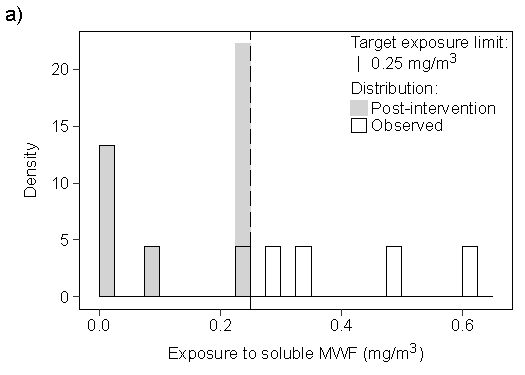
\includegraphics[keepaspectratio]{resources/intervention-density-witnin-combos-a.pdf}}

}

\end{minipage}%
%
\begin{minipage}{0.50\linewidth}

\subcaption{\label{fig-1b}}

\centering{

\pandocbounded{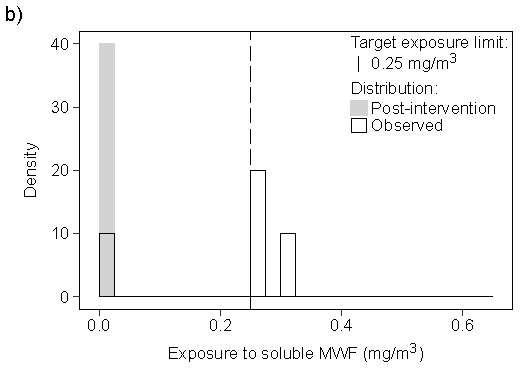
\includegraphics[keepaspectratio]{resources/intervention-density-witnin-combos-b.pdf}}

}

\end{minipage}%
\newline
\begin{minipage}{0.50\linewidth}

\subcaption{\label{fig-1c}}

\centering{

\pandocbounded{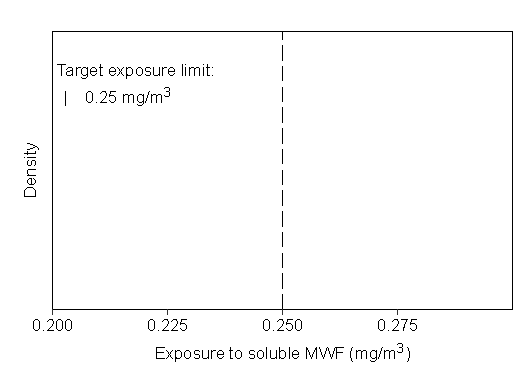
\includegraphics[keepaspectratio]{resources/intervention-density-witnin-combos-c.pdf}}

}

\end{minipage}%

\end{figure}%

\begin{table}

\caption{\label{tbl-1}Summary of population characteristics. Statistics
shown above the horizontal line are count (\%). Those shown below are
median (quartile 1, quartile 3).}

\centering{

\begin{tabular}{lrlrl}
  \toprule & \multicolumn{2}{c}{Study population} & \multicolumn{2}{c}{NHL Cases} \\ 
\cmidrule(lr){2-3}\cmidrule(lr){4-5}
% & Count & (\%) & Count & (\%) \\ 
 N (person-years) & 33,134 & (794,733) & 339 & (5,809) \\ 
   \midrule & Count & (\%)     & Count & (\%) \\
\midrule
Race &  &  &  &  \\ 
  \hspace{2em}White & 21,315 & (64\%) & 250 & (74\%) \\ 
  \hspace{2em}Black & 6,250 & (19\%) & 40 & (12\%) \\ 
  \hspace{2em}Unknown & 5,569 & (17\%) & 49 & (14\%) \\ 
  Sex &  &  &  &  \\ 
  \hspace{2em}Male & 28,640 & (86\%) & 297 & (88\%) \\ 
  \hspace{2em}Female & 4,494 & (14\%) & 42 & (12\%) \\ 
  Plant &  &  &  &  \\ 
  \hspace{2em}Plant 1 & 7,273 & (22\%) & 70 & (21\%) \\ 
  \hspace{2em}Plant 2 & 14,251 & (43\%) & 137 & (40\%) \\ 
  \hspace{2em}Plant 3 & 11,610 & (35\%) & 132 & (39\%) \\ 
  Ever exposed to MWFs &  &  &  &  \\ 
  \hspace{2em}Soluble & 29,010 & (88\%) & 299 & (88\%) \\ 
  \hspace{2em}Straight & 18,710 & (56\%) & 197 & (58\%) \\ 
  \hspace{2em}Synthetic & 11,824 & (36\%) & 111 & (33\%) \\ 
   \midrule & Median & (Q1, Q3) & Median & (Q1, Q3) \\
\midrule
Year of birth & 1941 & (1927, 1950) & 1935 & (1926, 1945) \\ 
  Year of hire & 1967 & (1953, 1976) & 1964 & (1953, 1971) \\ 
  Age at hire (years) & 23.6 & (20.0, 30.3) & 25.3 & (20.2, 32.9) \\ 
  Age at leaving work (years) & 45.2 & (31.8, 57.3) & 53.0 & (36.4, 60.4) \\ 
  Years at work & 15.2 & (7.0, 26.6) & 21.0 & (7.8, 29.9) \\ 
  Year of death & 2001 & (1994, 2009) & 2004 & (1998, 2010) \\ 
  Age at death (years) & 73.4 & (64.4, 81.3) & 73.0 & (66.3, 80.8) \\ 
  Cumulative exposurey) &  &  &  &  \\ 
  \hspace{2em}Soluble  & 4.33 & (1.71, 10.69) & 5.43 & (2.19, 14.33) \\ 
  \hspace{2em}Straight  & 0.67 & (0.21, 2.38) & 0.77 & (0.18, 3.52) \\ 
  \hspace{2em}Synthetic  & 0.44 & (0.15, 1.58) & 0.69 & (0.18, 1.91) \\ 
   \bottomrule
\end{tabular}

}

\end{table}%

\hfill\break

\begin{figure}

\caption{\label{fig-exposure}Median annual average daily exposure to
soluble, straight, and synthetic metalworking fluids among exposed
workers over time.}

\centering{

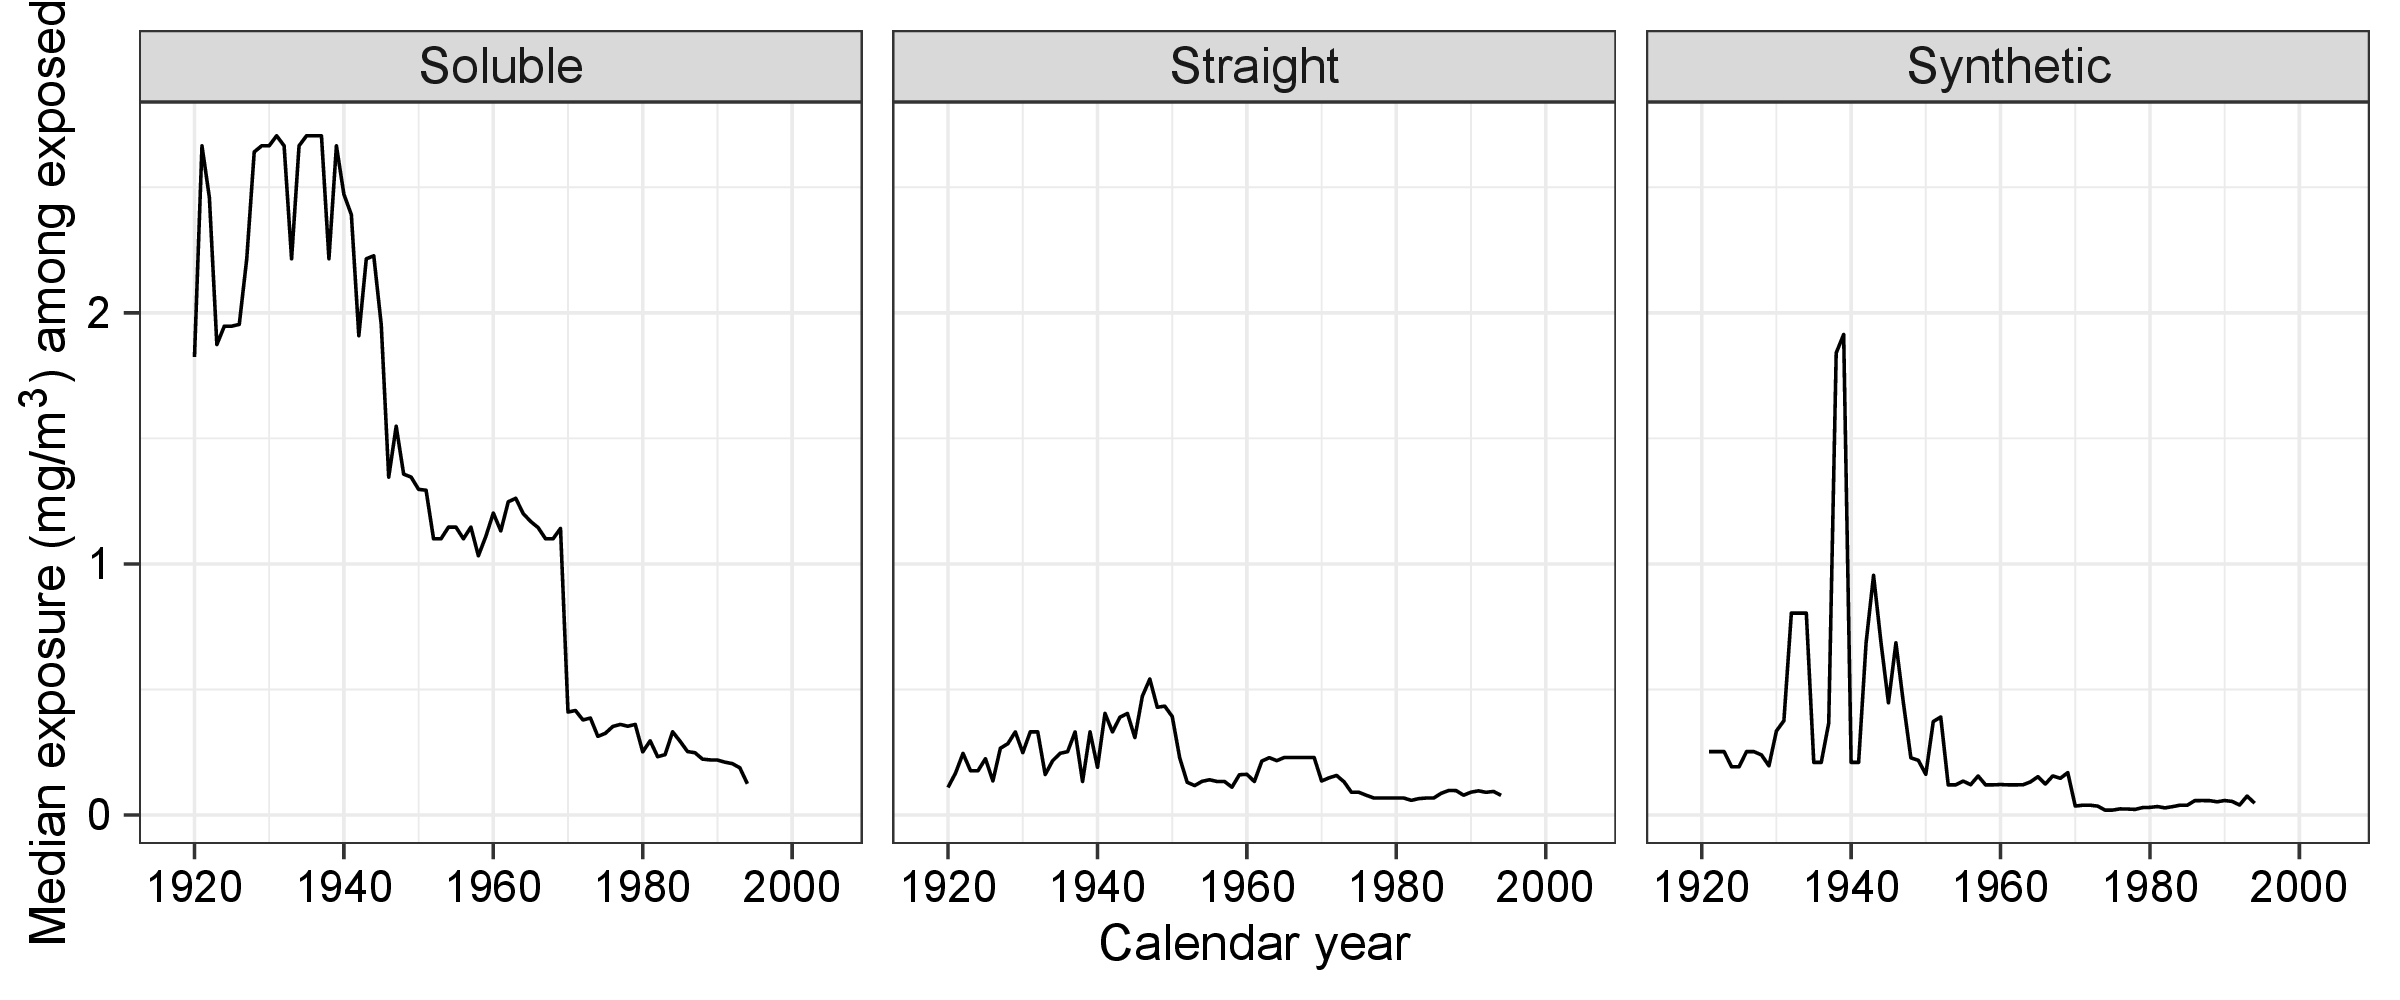
\includegraphics[width=6.5in,height=\textheight,keepaspectratio]{../../resources/images/exposure.png}

}

\end{figure}%

\begin{table}

\caption{\label{tbl-rd}Estimates of the counterfactual number of cases,
number of cases averted, and cumulative incidence ratios (CIR)
contrasting supportable interventions on annual average daily exposure
to soluble MWF to no intervention on exposure.}

\centering{

\begin{tabular}{lrlrlrl}
  \toprule
Target exposure limit (mg/m\textsuperscript{3}) & Cases & (95\% CI) & RD & (95\% CI) & CIR & (95\% CI) \\ 
  \midrule
None & 308 & (439, 555) &  &  &  &  \\ 
  2.0 & 280 & (317, 464) & 8.00 & (-103, 18) & 0.91 & (0.89, 1.13) \\ 
  1.0 & 277 & (306, 457) & 9.00 & (-110, 20) & 0.90 & (0.89, 1.13) \\ 
  0.5 & 268 & (296, 450) & 12.00 & (-102, 34) & 0.87 & (0.83, 1.09) \\ 
  0.25 & 260 & (286, 445) & 15.00 & (-99, 46) & 0.84 & (0.78, 1.06) \\ 
  0.05 & 238 & (262, 439) & 21.00 & (-79, 88) & 0.77 & (0.65, 0.97) \\ 
   \bottomrule
\end{tabular}

}

\end{table}%




\end{document}
